\begin{figure}[H] 
        \centering
        \begin{subfigure}[b]{0.45\linewidth}
            \centering
            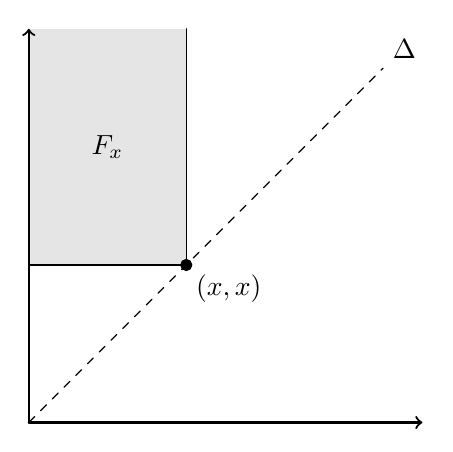
\begin{tikzpicture}[line cap=round, line join=round, x=1cm, y=1cm]
                
                \draw[thick,->] (0,0) -- (5,0);
                \draw[thick,->] (0,0) -- (0,5);
                \draw[dashed] (0,0) -- (4.5,4.5) node[above right] {$\Delta$};

                \draw[fill=black] (2, 2) circle (2pt) node[below right] {$(x, x)$}; 

                \draw (2, 2) -- (0, 2);
                \draw (2, 2) -- (2, 5);

                \fill[fill=black, fill opacity=0.1] (0, 5) -- (2, 5) -- (2, 2) -- (0, 2) -- cycle;
                \draw (1, 3.5) node {$F_x$};
                
            \end{tikzpicture}
            \caption{Homology modules of $f^{-1}(-\infty, x) $.}
        \end{subfigure}
        \hfill
        \begin{subfigure}[b]{0.45\linewidth}
            \centering
            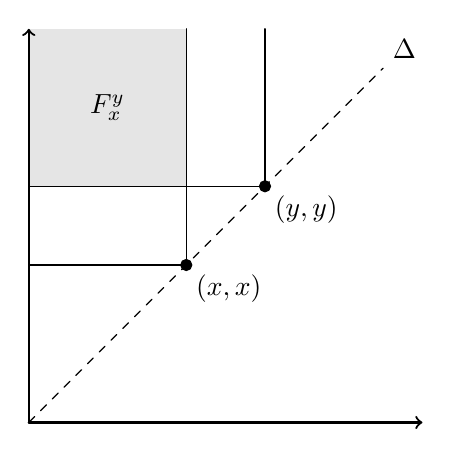
\begin{tikzpicture}[line cap=round, line join=round, x=1cm, y=1cm]
                
                \draw[thick,->] (0,0) -- (5,0);
                \draw[thick,->] (0,0) -- (0,5);
                \draw[dashed] (0,0) -- (4.5,4.5) node[above right] {$\Delta$};

                \draw[fill=black] (2, 2) circle (2pt) node[below right] {$(x, x)$}; 
                \draw[fill=black] (3,3) circle (2pt) node[below right] {$(y, y)$};

                \draw (2, 2) -- (0, 2);
                \draw (2, 2) -- (2, 5);

                \draw (3, 3) -- (0, 3);
                \draw (3, 3) -- (3, 5);

                \fill[fill=black, fill opacity=0.1] (0, 5) -- (2, 5) -- (2, 3) -- (0, 3) -- cycle;
                \draw (1, 4) node {$F_x^y$};
                
            \end{tikzpicture}
            \caption{Image of $ F_x $ in $ F_y $.}
        \end{subfigure}
        \begin{subfigure}[b]{0.45\linewidth}
            \centering
            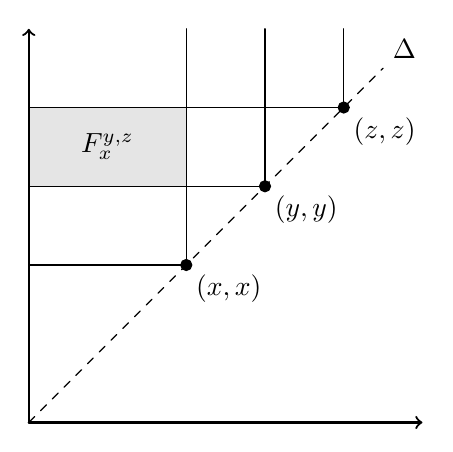
\begin{tikzpicture}[line cap=round, line join=round, x=1cm, y=1cm]
                
                \draw[thick,->] (0,0) -- (5,0);
                \draw[thick,->] (0,0) -- (0,5);
                \draw[dashed] (0,0) -- (4.5,4.5) node[above right] {$\Delta$};

                \draw[fill=black] (2, 2) circle (2pt) node[below right] {$(x, x)$}; 
                \draw[fill=black] (3,3) circle (2pt) node[below right] {$(y, y)$}; 
                \draw[fill=black] (4,4) circle (2pt) node[below right] {$(z, z)$};

                \draw (2, 2) -- (0, 2);
                \draw (2, 2) -- (2, 5);

                \draw (3, 3) -- (0, 3);
                \draw (3, 3) -- (3, 5);

                \draw (4, 4) -- (0, 4);
                \draw (4, 4) -- (4, 5);
                
                \fill[fill=black, fill opacity=0.1] (0, 4) -- (2, 4) -- (2, 3) -- (0, 3) -- cycle;
                \draw (1, 3.5) node {$F_x^{y, z}$};

            \end{tikzpicture}
            \caption{Kernel of the surjection $ F_x^y \to F_x^z $.}
        \end{subfigure}
        \hfill
        \begin{subfigure}[b]{0.45\linewidth}
            \centering
            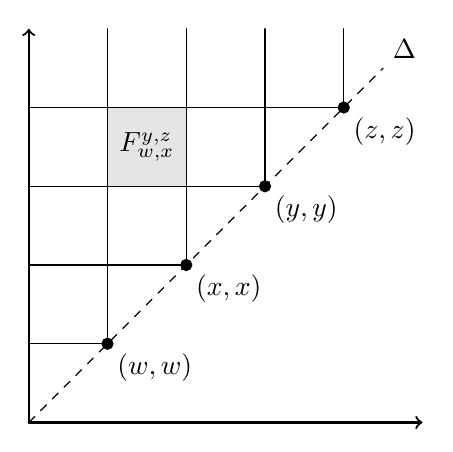
\begin{tikzpicture}[line cap=round, line join=round, x=1cm, y=1cm]
                
                \draw[thick,->] (0,0) -- (5,0);
                \draw[thick,->] (0,0) -- (0,5);
                \draw[dashed] (0,0) -- (4.5,4.5) node[above right] {$\Delta$};

                \draw[fill=black] (2, 2) circle (2pt) node[below right] {$(x, x)$}; 
                \draw[fill=black] (3,3) circle (2pt) node[below right] {$(y, y)$}; 
                \draw[fill=black] (4,4) circle (2pt) node[below right] {$(z, z)$}; 
                \draw[fill=black] (1,1) circle (2pt) node[below right] {$(w, w)$}; 

                \draw (2, 2) -- (0, 2);
                \draw (2, 2) -- (2, 5);

                \draw (3, 3) -- (0, 3);
                \draw (3, 3) -- (3, 5);

                \draw (4, 4) -- (0, 4);
                \draw (4, 4) -- (4, 5);

                \draw (1, 1) -- (0, 1);
                \draw (1, 1) -- (1, 5);

                \fill[fill=black, fill opacity=0.1] (1, 4) -- (2, 4) -- (2, 3) -- (1, 3) -- cycle;
                \draw (1.5, 3.5) node {$F_{w,x}^{y, z}$};
                
            \end{tikzpicture}
            \caption{Quotient of $ F_x^{y, z} $ and $ F_w^{y, z} $.}
        \end{subfigure}
        \caption{Persistent homology notation.}
        \label{fig:homology-modules}
    \end{figure}